\section*{Circuitos combinacionais II}

\frame{
	\frametitle{Códigos binários - BCD 8421}
	\begin{block}{BCD 8241}
		\begin{itemize}
			\item BCD: \textit{binary coded decimal}.
			\item Técnica mais simples e normal de ser utilizada -- \textbf{natural}.
			\item Cada dígito binário é representado pelo seu correspondente binário de 4 dígitos.
			\item 8421 indica os "pesos" de cada algarismo no sistema binário.
			\item A grande vantagem do sistema BCD 8421 é a facilidade  entre homem-máquina.
			\item O código BCD, no entanto, é menos eficiente que o código binário puro, pois são usados \textbf{mais bits }para se representar um determinado valor.
		\end{itemize}
	\end{block}
}

\frame{
	\frametitle{Códigos binários - BCD 8421}
	
	\renewcommand{\arraystretch}{1}
	\centering
	\begin{adjustbox}{totalheight=0.75\textheight-2\baselineskip}
	\centering
	\begin{tabular}{c|cccc}
		\toprule
		\multirow{2}{*}{\makecell{\normalsize Decimal}} & \multicolumn{4}{c}{\makecell{\normalsize BCD 8421}} \\ \cmidrule{2-5}
		  & A & B & C & D \\ \midrule
		0 & 0 & 0 & 0 & 0 \\
		1 & 0 & 0 & 0 & 1 \\
		2 & 0 & 0 & 1 & 0 \\
		3 & 0 & 0 & 1 & 1 \\
		4 & 0 & 1 & 0 & 0 \\
		5 & 0 & 1 & 0 & 1 \\
		6 & 0 & 1 & 1 & 0 \\
		7 & 0 & 1 & 1 & 1 \\
		8 & 1 & 0 & 0 & 0 \\
		9 & 1 & 0 & 0 & 1 \\ \bottomrule
	\end{tabular}
	\end{adjustbox}

	\begin{block}{}
		\begin{itemize}
			\setlength\itemsep{0.25em}
			\item $ \mathsmaller{10 = 0001\; \! 0000} $
			\item $ \mathsmaller{11 = 0001\; \! 0001} $
			\item $ \mathsmaller{\ldots} $
			\item $ \mathsmaller{15 = 0001\; \! 0101} $
		\end{itemize}
	\end{block}
}

\frame{
	\frametitle{Códigos binários - BCD 7421}
	
%	\renewcommand{\arraystretch}{1}
	\centering
	\begin{adjustbox}{totalheight=1\textheight-2\baselineskip}
		\centering
		\begin{tabular}{c|cccc}
			\toprule
			\multirow{2}{*}{\makecell{\normalsize Decimal}} & \multicolumn{4}{c}{\makecell{\normalsize BCD 7421}} \\ \cmidrule{2-5}
			& A & B & C & D \\ \midrule
			0 & 0 & 0 & 0 & 0 \\
			1 & 0 & 0 & 0 & 1 \\
			2 & 0 & 0 & 1 & 0 \\
			3 & 0 & 0 & 1 & 1 \\
			4 & 0 & 1 & 0 & 0 \\
			5 & 0 & 1 & 0 & 1 \\
			6 & 0 & 1 & 1 & 0 \\
			7 & 1 & 0 & 0 & 0 \\
			8 & 1 & 0 & 0 & 1 \\
			9 & 1 & 0 & 1 & 0 \\ \bottomrule
		\end{tabular}
	\end{adjustbox}
}

\frame{
	\frametitle{Códigos binários - Excesso 3}
	
	\begin{block}{}
		\begin{itemize}
			\item Transformação do número decimal no binário correspondente somando-se 3 unidades.
			\item É obtido adiantando o código BCD três vezes.
			\item Neste modelo há apenas de zero a nove decimal.
			\item Apresenta algumas vantagens nas operações matemáticas - utilizado em circuitos aritméticos.
		\end{itemize}
	\end{block}
}

\frame{
	\frametitle{Códigos binários - Excesso 3}
	
%	\renewcommand{\arraystretch}{1}
	\centering
	\begin{adjustbox}{totalheight=1\textheight-2\baselineskip}
		\centering
		\begin{tabular}{c|cccc}
			\toprule
			\multirow{2}{*}{\makecell{\normalsize Decimal}} & \multicolumn{4}{c}{\makecell{\normalsize Excesso 3}} \\ \cmidrule{2-5}
			& A & B & C & D \\ \midrule
			0 & 0 & 0 & 1 & 1 \\
			1 & 0 & 1 & 0 & 0 \\
			2 & 0 & 1 & 0 & 1 \\
			3 & 0 & 1 & 1 & 0 \\
			4 & 0 & 1 & 1 & 1 \\
			5 & 1 & 0 & 0 & 0 \\
			6 & 1 & 0 & 0 & 1 \\
			7 & 1 & 0 & 1 & 0 \\
			8 & 1 & 0 & 1 & 1 \\
			9 & 1 & 1 & 0 & 0 \\ \bottomrule
		\end{tabular}
	\end{adjustbox}
%	\centerline{\includegraphics[width=0.4\linewidth]{Figuras/Ch8/excesso3.PNG}}
}

\frame{
	\frametitle{Códigos binários - Gray}
	\begin{block}{}
		\begin{itemize}
			\item De um número para o outro apenas \textbf{um bit }varia.
			\item A cada linha o número binário é variado em um algarismo de forma que não se repita nenhum anterior.
			\item Utilizado no K-map.
			\item Sua estrutura facilita a detecção de erros.
		\end{itemize}
	\end{block}
}

\frame{
	\frametitle{Códigos binários - Gray}
	
%	\renewcommand{\arraystretch}{1}
	\centering
	\begin{adjustbox}{totalheight=1\textheight-2\baselineskip}
		\centering
		\begin{tabular}{c|cccc}
			\toprule
			\multirow{2}{*}{\makecell{\normalsize Decimal}} & \multicolumn{4}{c}{\makecell{\normalsize Gray}} \\ \cmidrule{2-5}
			  & A & B & C & D \\ \midrule
			0 & 0 & 0 & 0 & 0 \\
			1 & 0 & 0 & 0 & 1 \\
			2 & 0 & 0 & 1 & 1 \\
			3 & 0 & 0 & 1 & 0 \\
			4 & 0 & 1 & 1 & 0 \\
			5 & 0 & 1 & 1 & 1 \\
			6 & 0 & 1 & 0 & 1 \\
			7 & 0 & 1 & 0 & 0 \\
			8 & 1 & 1 & 0 & 0 \\
			9 & 1 & 1 & 0 & 1 \\
			10& 1 & 1 & 1 & 1 \\
			11& 1 & 1 & 1 & 0 \\
			12& 1 & 0 & 1 & 0 \\
			13& 1 & 0 & 1 & 1 \\
			14& 1 & 0 & 0 & 1 \\
			15& 1 & 0 & 0 & 0 \\ \bottomrule
		\end{tabular}
	\end{adjustbox}
%	\centerline{\includegraphics[width=0.4\linewidth]{Figuras/Ch8/gray.PNG}}
}

\frame{
	\frametitle{Códigos binários - Johnson}
	
	\begin{block}{}
		\begin{itemize}
			\item Possui cinco dígitos binários.
			\item Cada código possui apenas um bit diferente do seu sucessor.
			\item Sua vantagem é a facilidade de gerar palavras código.
		\end{itemize}
	\end{block}
}

\frame{
	\frametitle{Códigos binários - Johnson}
	
%	\renewcommand{\arraystretch}{1}
	\centering
	\begin{adjustbox}{totalheight=1\textheight-2\baselineskip}
		\centering
		\begin{tabular}{c|ccccc}
			\toprule
			\multirow{2}{*}{\makecell{\normalsize Decimal}} & \multicolumn{5}{c}{\makecell{\normalsize Johnson}} \\ \cmidrule{2-6}
			  & A & B & C & D & E \\ \midrule
			0 & 0 & 0 & 0 & 0 & 0 \\
			1 & 0 & 0 & 0 & 0 & 1 \\
			2 & 0 & 0 & 0 & 1 & 1 \\
			3 & 0 & 0 & 1 & 1 & 1 \\
			4 & 0 & 1 & 1 & 1 & 1 \\
			5 & 1 & 1 & 1 & 1 & 1 \\
			6 & 1 & 1 & 1 & 1 & 0 \\
			7 & 1 & 1 & 1 & 0 & 0 \\
			8 & 1 & 1 & 0 & 0 & 0 \\
			9 & 1 & 0 & 0 & 0 & 0 \\ \bottomrule
		\end{tabular}
	\end{adjustbox}
%	\centerline{\includegraphics[width=0.5\linewidth]{Figuras/Ch8/johnson.PNG}}
}

\frame{
	\frametitle{Códigos binários - 9876543210}
	
	\begin{block}{}
		\begin{itemize}
			\item Decodificação de ``uma saída de 10''.
			\item Um único bit será 1, enquanto os demais serão 0
			\item O valor 1 assume a posição correspondente ao número decimal
		\end{itemize}
	\end{block}

}

\frame{
	\frametitle{Códigos binários - 9876543210}
	
%	\renewcommand{\arraystretch}{1}
	\centering
	\begin{adjustbox}{totalheight=1\textheight-2\baselineskip}
		\centering
		\begin{tabular}{c|cccccccccc}
			\toprule
			\multirow{2}{*}{\makecell{\normalsize Decimal}} & \multicolumn{10}{c}{\makecell{\normalsize 9876543210}} \\ \cmidrule{2-11}
			  & 9 & 8 & 7 & 6 & 5 & 4 & 3 & 2 & 1 & 0 \\ \midrule
			0 & 0 & 0 & 0 & 0 & 0 & 0 & 0 & 0 & 0 & 1 \\
			1 & 0 & 0 & 0 & 0 & 0 & 0 & 0 & 0 & 1 & 0 \\
			2 & 0 & 0 & 0 & 0 & 0 & 0 & 0 & 1 & 0 & 0 \\
			3 & 0 & 0 & 0 & 0 & 0 & 0 & 1 & 0 & 0 & 0 \\
			4 & 0 & 0 & 0 & 0 & 0 & 1 & 0 & 0 & 0 & 0 \\
			5 & 0 & 0 & 0 & 0 & 1 & 0 & 0 & 0 & 0 & 0 \\
			6 & 0 & 0 & 0 & 1 & 0 & 0 & 0 & 0 & 0 & 0 \\
			7 & 0 & 0 & 1 & 0 & 0 & 0 & 0 & 0 & 0 & 0 \\
			8 & 0 & 1 & 0 & 0 & 0 & 0 & 0 & 0 & 0 & 0 \\
			9 & 1 & 0 & 0 & 0 & 0 & 0 & 0 & 0 & 0 & 0 \\ \bottomrule
		\end{tabular}
	\end{adjustbox}
%	\centerline{\includegraphics[width=0.7\linewidth]{Figuras/Ch8/9876543210.PNG}}

}

\frame{
	\frametitle{Codificadores e decodificadores}
	
	\begin{block}{}
		\begin{itemize}
			\item \alert{\textbf{Codificador}} é um circuito combinacional que torna possível a passagem de um código conhecido para um desconhecido.
			\item Por outro lado, \alert{\textbf{decodificador}} faz a operação inversa: passa um código desconhecido para um conhecido. 
		\end{itemize}
	\end{block}
	\centerline{\includegraphics[width=0.4\linewidth]{Figuras/Ch8/calculadora.png}}
}

\frame{
	\frametitle{Codificadores e decodificadores}
	
%	\centerline{\includegraphics[width=0.6\linewidth]{Figuras/Ch8/calculadora2.png}}

	\centering
	\scalebox{0.6}{

\tikzset{every picture/.style={line width=0.75pt}} %set default line width to 0.75pt        

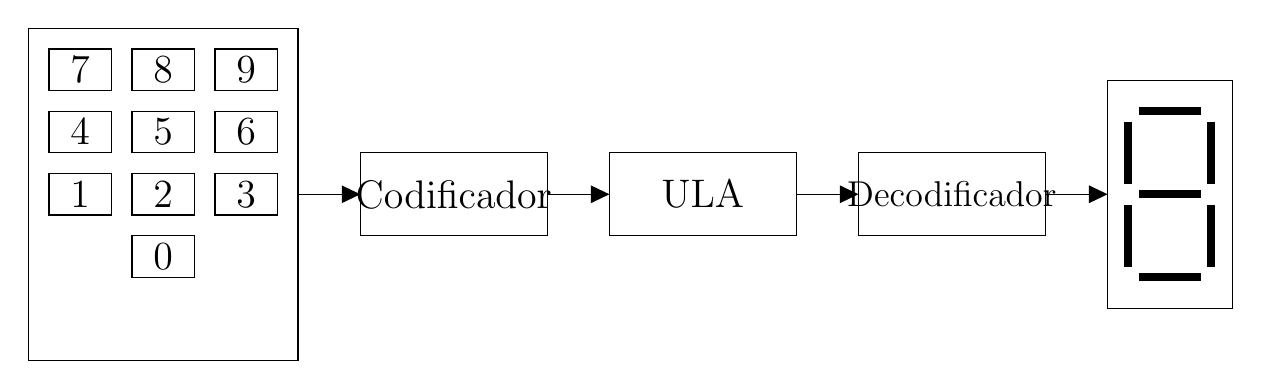
\begin{tikzpicture}[x=0.75pt,y=0.75pt,yscale=-1,xscale=1]
%uncomment if require: \path (0,300); %set diagram left start at 0, and has height of 300

%Shape: Rectangle [id:dp8798188650405219] 
\draw   (30,50) -- (160,50) -- (160,210) -- (30,210) -- cycle ;
%Shape: Rectangle [id:dp593444354888008] 
\draw   (40,60) -- (70,60) -- (70,80) -- (40,80) -- cycle ;
%Shape: Rectangle [id:dp4412846627526852] 
\draw   (80,60) -- (110,60) -- (110,80) -- (80,80) -- cycle ;
%Shape: Rectangle [id:dp2343273962035186] 
\draw   (120,60) -- (150,60) -- (150,80) -- (120,80) -- cycle ;
%Shape: Rectangle [id:dp05777918912875246] 
\draw   (40,90) -- (70,90) -- (70,110) -- (40,110) -- cycle ;
%Shape: Rectangle [id:dp9955010424516375] 
\draw   (80,90) -- (110,90) -- (110,110) -- (80,110) -- cycle ;
%Shape: Rectangle [id:dp24021539717259266] 
\draw   (120,90) -- (150,90) -- (150,110) -- (120,110) -- cycle ;
%Shape: Rectangle [id:dp36169684584711925] 
\draw   (40,120) -- (70,120) -- (70,140) -- (40,140) -- cycle ;
%Shape: Rectangle [id:dp7232437677097003] 
\draw   (80,120) -- (110,120) -- (110,140) -- (80,140) -- cycle ;
%Shape: Rectangle [id:dp6884539525496838] 
\draw   (120,120) -- (150,120) -- (150,140) -- (120,140) -- cycle ;
%Shape: Rectangle [id:dp9961423077173726] 
\draw   (80,150) -- (110,150) -- (110,170) -- (80,170) -- cycle ;
%Shape: Rectangle [id:dp6643057105712631] 
\draw   (190,110) -- (280,110) -- (280,150) -- (190,150) -- cycle ;
%Shape: Rectangle [id:dp7094011053258715] 
\draw   (550,75) -- (610,75) -- (610,185) -- (550,185) -- cycle ;
%Shape: Rectangle [id:dp2693438921699036] 
\draw   (310,110) -- (400,110) -- (400,150) -- (310,150) -- cycle ;
%Shape: Rectangle [id:dp3654960401722005] 
\draw   (430,110) -- (520,110) -- (520,150) -- (430,150) -- cycle ;
%Straight Lines [id:da6667328032348829] 
\draw    (160,130) -- (188,130) ;
\draw [shift={(190,130)}, rotate = 180] [fill={rgb, 255:red, 0; green, 0; blue, 0 }  ][line width=0.75]  [draw opacity=0] (8.93,-4.29) -- (0,0) -- (8.93,4.29) -- cycle    ;

%Straight Lines [id:da5165651690517046] 
\draw    (280,130) -- (308,130) ;
\draw [shift={(310,130)}, rotate = 180] [fill={rgb, 255:red, 0; green, 0; blue, 0 }  ][line width=0.75]  [draw opacity=0] (8.93,-4.29) -- (0,0) -- (8.93,4.29) -- cycle    ;

%Straight Lines [id:da17751850693095572] 
\draw    (400,130) -- (428,130) ;
\draw [shift={(430,130)}, rotate = 180] [fill={rgb, 255:red, 0; green, 0; blue, 0 }  ][line width=0.75]  [draw opacity=0] (8.93,-4.29) -- (0,0) -- (8.93,4.29) -- cycle    ;

%Straight Lines [id:da4998570413390182] 
\draw [color={rgb, 255:red, 0; green, 0; blue, 0 }  ,draw opacity=1 ][line width=3]    (560,95) -- (560,125) ;


%Straight Lines [id:da05287212083080073] 
\draw [color={rgb, 255:red, 0; green, 0; blue, 0 }  ,draw opacity=1 ][line width=3]    (600,95) -- (600,125) ;


%Straight Lines [id:da9146969001147236] 
\draw [color={rgb, 255:red, 0; green, 0; blue, 0 }  ,draw opacity=1 ][line width=3]    (560,135) -- (560,165) ;


%Straight Lines [id:da37610179690179124] 
\draw [color={rgb, 255:red, 0; green, 0; blue, 0 }  ,draw opacity=1 ][line width=3]    (600,135) -- (600,165) ;


%Straight Lines [id:da2798262228013664] 
\draw [color={rgb, 255:red, 0; green, 0; blue, 0 }  ,draw opacity=1 ][line width=3]    (595,130) -- (565,130) ;


%Straight Lines [id:da15184615547446478] 
\draw [color={rgb, 255:red, 0; green, 0; blue, 0 }  ,draw opacity=1 ][line width=3]    (595,90) -- (565,90) ;


%Straight Lines [id:da20609816632014244] 
\draw [color={rgb, 255:red, 0; green, 0; blue, 0 }  ,draw opacity=1 ][line width=3]    (595,170) -- (565,170) ;


%Straight Lines [id:da16937059284664002] 
\draw    (520,130) -- (548,130) ;
\draw [shift={(550,130)}, rotate = 180] [fill={rgb, 255:red, 0; green, 0; blue, 0 }  ][line width=0.75]  [draw opacity=0] (8.93,-4.29) -- (0,0) -- (8.93,4.29) -- cycle    ;


% Text Node
\draw (135,70) node   {\Large $9$};
% Text Node
\draw (95,70) node   {\Large $8$};
% Text Node
\draw (55,70) node   {\Large $7$};
% Text Node
\draw (135,100) node   {\Large $6$};
% Text Node
\draw (135,130) node   {\Large $3$};
% Text Node
\draw (95,160) node   {\Large $0$};
% Text Node
\draw (95,130) node   {\Large $2$};
% Text Node
\draw (95,100) node   {\Large $5$};
% Text Node
\draw (55,100) node   {\Large $4$};
% Text Node
\draw (55,130) node   {\Large $1$};
% Text Node
\draw (235,130) node  [align=left] {\Large Codificador};
% Text Node
\draw (355,130) node  [align=left] {\Large ULA};
% Text Node
\draw (475,130) node [scale=0.9] [align=left] {\Large Decodificador};


\end{tikzpicture}
}

	\begin{block}{Atenção:}
		\begin{itemize}
			\item Depende do referencial.
			\item Para o usuário:
			      \begin{itemize}
				      \item Sistema de entrada: codificador.
				      \item Sistema de saída: decodificador.
			      \end{itemize}
			\item Para a máquina:
			      \begin{itemize}
				      \item Sistema de entrada: decodificador.
				      \item Sistema de saída: codificador.
			      \end{itemize}
		\end{itemize}
	\end{block}
}

\frame{
	\frametitle{Codificadores e decodificadores - Projeto \#01 - calculadora}
	\begin{block}{}
		\begin{itemize}
			\item Primeira parte: codificador decimal-binário
		\end{itemize}
	\end{block}

	\centering
	\scalebox{0.75}{\setmyunit{2cm}
		\begin{circuitikz}[scale=0.9]
			\node[ground] (g) at (0,0) {};
			\draw (g) -- ++(0,0.3) to[short, *-*] ++(0,0.7) to[short, -*] ++(0,0.5) -- ++(0,0.5) to[nopb=ch0] ++(1,0) ++(-1,-0.5) to[nopb=ch1] ++(1,0) ++(-1,-0.5) to[nopb=ch2] ++(1,0) ++(-1,-0.7) to[nopb=ch9,name=cc] ++(1,0) ++(0,-0.2) rectangle node[text width=1.8cm] {Codificador decimal/ binário} ++(2,2.1) ++(0,-0.5) -- ++(1,0) node[right] {$ A $} ++(-1,-0.4) -- ++(1,0) node[right] {$ B $} ++(-1,-0.4) -- ++(1,0) node[right] {$ C $} ++(-1,-0.4) -- ++(1,0) node[right] {$ D $};
			\node[above=0.7cm] at (cc) {$ \vdots $};
	\end{circuitikz}}

%	\centerline{\includegraphics[width=0.6\linewidth]{Figuras/Ch8/calculadora3.PNG}}

	\begin{block}{Codificador decimal-binário}
		\begin{itemize}
			\item Entrada: chaves de 0 a 9
			\item Saída: 4 bits em BCD 8421
			\item Chave fechada equivale a nível 0 - problema TTL.
		\end{itemize}
	\end{block}
}

\frame{
	\frametitle{Codificadores e decodificadores - Projeto \#01 - calculadora}
	
	\renewcommand{\arraystretch}{1.2}
	\centering
	\begin{adjustbox}{totalheight=1\textheight-2\baselineskip}
		\centering
		\begin{tabular}{c|cccc}
			\toprule
			\multirow{2}{*}{\makecell{\normalsize Decimal}} & \multicolumn{4}{c}{\makecell{\normalsize BCD 8421}} \\ \cmidrule{2-5}
			& A & B & C & D \\ \midrule
			Ch0 & 0 & 0 & 0 & 0 \\
			Ch1 & 0 & 0 & 0 & 1 \\
			Ch2 & 0 & 0 & 1 & 0 \\
			Ch3 & 0 & 0 & 1 & 1 \\
			Ch4 & 0 & 1 & 0 & 0 \\
			Ch5 & 0 & 1 & 0 & 1 \\
			Ch6 & 0 & 1 & 1 & 0 \\
			Ch7 & 0 & 1 & 1 & 1 \\
			Ch8 & 1 & 0 & 0 & 0 \\
			Ch9 & 1 & 0 & 0 & 1 \\ \bottomrule
		\end{tabular}
	\end{adjustbox}
	
%	\centerline{\includegraphics[width=0.6\linewidth]{Figuras/Ch8/calculadora4.PNG}}
}

\frame{
	\frametitle{Codificadores e decodificadores - Projeto \#01 - calculadora}
	\begin{block}{Lembre-se:}
		\begin{itemize}
			\item Chave fechada equivale a nível 0 - problema TTL.
	      	\item Utilização de uma porta NAND em cada saída
	     	\item Fornece nível 1 quando qualquer entrada for 0 (chave fechada).
	    \end{itemize}
	\end{block}
	\centerline{\includegraphics[width=0.6\linewidth]{Figuras/Ch8/calculadora5.PNG}}
}

\frame{
	\frametitle{Codificadores e decodificadores - Projeto \#01 - calculadora}
	\begin{block}{}
		\begin{itemize}
			\item Segunda parte: decodificador binário-decimal
		\end{itemize}
	\end{block}

	\setmyunit{2cm}
	
	\centering
	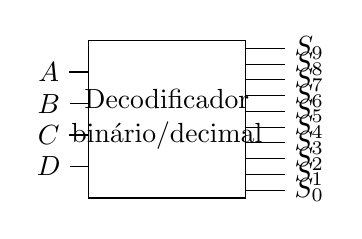
\begin{tikzpicture}
		\node (a) at (0,0.6) {$ A $};
		\node (b) at (0,0.2) {$ B $};
		\node (c) at (0,-0.2) {$ C $};
		\node (d) at (0,-0.6) {$ D $};
		
		\draw (0.5,-1) rectangle node[midway, text width=3cm, align=center] {Decodificador binário/decimal} ++(2,2)
		(a) -- ++(0.5,0)
		(b) -- ++(0.5,0)
		(c) -- ++(0.5,0)
		(d) -- ++(0.5,0);
		
%		\foreach \x/\y in {9/0.9,8/0.7,...,0/-0.9}
%			{\draw (3,\y) node[right] {$ S_\x $} -- ++(-0.5,0);}
		
		\draw (3,0.9) node[right] {$ S_9 $} -- ++(-0.5,0);
		\draw (3,0.7) node[right] {$ S_8 $} -- ++(-0.5,0);
		\draw (3,0.5) node[right] {$ S_7 $} -- ++(-0.5,0);
		\draw (3,0.3) node[right] {$ S_6 $} -- ++(-0.5,0);
		\draw (3,0.1) node[right] {$ S_5 $} -- ++(-0.5,0);
		\draw (3,-0.1) node[right] {$ S_4 $} -- ++(-0.5,0);
		\draw (3,-0.3) node[right] {$ S_3 $} -- ++(-0.5,0);
		\draw (3,-0.5) node[right] {$ S_2 $} -- ++(-0.5,0);
		\draw (3,-0.7) node[right] {$ S_1 $} -- ++(-0.5,0);
		\draw (3,-0.9) node[right] {$ S_0 $} -- ++(-0.5,0);
	\end{tikzpicture}
%	\centerline{\includegraphics[width=0.6\linewidth]{Figuras/Ch8/calculadora6.PNG}}

	\begin{block}{Decodificador decimal-binário}
		\begin{itemize}
			\item Entrada: 4 bits em BCD 8421
			\item Saída: Código 9876543210
		\end{itemize}
	\end{block}
}

\frame{
	\frametitle{Codificadores e decodificadores - Projeto \#01 - calculadora}
	
	\renewcommand{\arraystretch}{1.2}
	\centering
	\resizebox{\textwidth}{!}{
		\centering
		\begin{tabular}{cccc|cccccccccc}
			\toprule
			\multicolumn{4}{c|}{\makecell{\normalsize BCD 8421}} & \multicolumn{10}{c}{\makecell{\normalsize Código 9876543210}} \\ \midrule %\cmidrule(r{1.2em}){1-4}\cmidrule(l{-0.2em}){5-14}
			$ A $ & $ B $ & $ C $ & $ D $ & $ S_9 $ & $ S_8 $ & $ S_7 $ & $ S_6 $ & $ S_5 $ & $ S_4 $ & $ S_3 $ & $ S_2 $ & $ S_1 $ & $ S_0 $ \\ \midrule
			0 & 0 & 0 & 0 & 0 & 0 & 0 & 0 & 0 & 0 & 0 & 0 & 0 & 1 \\
			0 & 0 & 0 & 1 & 0 & 0 & 0 & 0 & 0 & 0 & 0 & 0 & 1 & 0\\
			0 & 0 & 1 & 0 & 0 & 0 & 0 & 0 & 0 & 0 & 0 & 1 & 0 & 0\\
			0 & 0 & 1 & 1 & 0 & 0 & 0 & 0 & 0 & 0 & 1 & 0 & 0 & 0\\
			0 & 1 & 0 & 0 & 0 & 0 & 0 & 0 & 0 & 1 & 0 & 0 & 0 & 0\\
			0 & 1 & 0 & 1 & 0 & 0 & 0 & 0 & 1 & 0 & 0 & 0 & 0 & 0\\
			0 & 1 & 1 & 0 & 0 & 0 & 0 & 1 & 0 & 0 & 0 & 0 & 0 & 0\\
			0 & 1 & 1 & 1 & 0 & 0 & 1 & 0 & 0 & 0 & 0 & 0 & 0 & 0\\
			1 & 0 & 0 & 0 & 0 & 1 & 0 & 0 & 0 & 0 & 0 & 0 & 0 & 0\\
			1 & 0 & 0 & 1 & 1 & 0 & 0 & 0 & 0 & 0 & 0 & 0 & 0 & 0\\ \bottomrule
		\end{tabular}
	}
%	\centerline{\includegraphics[width=0.9\linewidth]{Figuras/Ch8/calculadora7.PNG}}
}

\frame{
	\frametitle{Codificadores e decodificadores - Projeto \#01 - calculadora}
	\begin{block}{Agora...}
		\begin{itemize}
			\item Monta-se o Mapa de Karnaugh para cada uma das saídas da tabela.
			\item Codigo BCD 8421 só vai até o 9 - demais casos: condição irrelevante
		\end{itemize}
	\end{block}
}


\frame{
\frametitle{Codificadores e decodificadores - Projeto \#01 - calculadora}
\begin{center}
\scalebox{0.9}{
	\begin{karnaugh-map}[4][4][1][$CD$][$AB$]
	\manualterms{0,0,0,0,0,0,0,0,0,1,X,X,X,X,X,X}
	\implicant{13}{11}
	%\implicant{7}{6}
	%\implicantedge{0}{1}{8}{9}
	%\implicantcorner
	%\implicantedge{4}{12}{6}{14}
	\end{karnaugh-map}
}

\end{center}

\vspace{-0.5cm}

\begin{block}{Expressão simplificada}
\[ S_9= {\color{red} A \cdot  D}\]
\end{block}
}

\frame{
\frametitle{Codificadores e decodificadores - Projeto \#01 - calculadora}
\begin{center}
\scalebox{0.9}{
	\begin{karnaugh-map}[4][4][1][$CD$][$AB$]
	\manualterms{0,0,0,0,0,0,0,0,1,0,X,X,X,X,X,X}
	%\implicant{15}{9}
	%\implicant{7}{6}
	\implicantedge{12}{8}{14}{10}
	%\implicantcorner
	%\implicantedge{4}{12}{6}{14}
	\end{karnaugh-map}
}

\end{center}

\vspace{-0.5cm}

\begin{block}{Expressão simplificada}
\[ S_8 = {\color{red} A\cdot \notted{D}} \]
\end{block}
}

\frame{
\frametitle{Codificadores e decodificadores - Projeto \#01 - calculadora}
\begin{center}
\scalebox{0.9}{
	\begin{karnaugh-map}[4][4][1][$CD$][$AB$]
	\manualterms{0,0,0,0,0,0,0,1,0,0,X,X,X,X,X,X}
	%\implicant{15}{9}
	\implicant{7}{15}
	%\implicantedge{0}{1}{8}{9}
	%\implicantcorner
	%\implicantedge{4}{12}{6}{14}
	\end{karnaugh-map}
}

\end{center}

\vspace{-0.5cm}

\begin{block}{Expressão simplificada}
\[ S_7 =  {\color{red} B\cdot C\cdot D}\]
\end{block}
}
\frame{
\frametitle{Codificadores e decodificadores - Projeto \#01 - calculadora}
\begin{center}
\scalebox{0.9}{
	\begin{karnaugh-map}[4][4][1][$CD$][$AB$]
	\manualterms{0,0,0,0,0,0,1,0,0,0,X,X,X,X,X,X}
	%\implicant{15}{9}
	\implicant{6}{14}
	%\implicantedge{0}{1}{8}{9}
	%\implicantcorner
	%\implicantedge{4}{12}{6}{14}
	\end{karnaugh-map}
}

\end{center}

\vspace{-0.5cm}

\begin{block}{Expressão simplificada}
\[ S_6 = {\color{red} B\cdot C\cdot \notted{D}} \]
\end{block}
}

\frame{
\frametitle{Codificadores e decodificadores - Projeto \#01 - calculadora}
\begin{center}
\scalebox{0.9}{
	\begin{karnaugh-map}[4][4][1][$CD$][$AB$]
	\manualterms{0,0,0,0,0,1,0,0,0,0,X,X,X,X,X,X}
	%\implicant{15}{9}
	\implicant{5}{13}
	%\implicantedge{0}{1}{8}{9}
	%\implicantcorner
	%\implicantedge{4}{12}{6}{14}
	\end{karnaugh-map}
}

\end{center}

\vspace{-0.5cm}

\begin{block}{Expressão simplificada}
\[ S_5 = {\color{red} B\cdot \notted{C}\cdot D} \]
\end{block}
}

\frame{
\frametitle{Codificadores e decodificadores - Projeto \#01 - calculadora}
\begin{center}
\scalebox{0.9}{
	\begin{karnaugh-map}[4][4][1][$CD$][$AB$]
	\manualterms{0,0,0,0,1,0,0,0,0,0,X,X,X,X,X,X}
	%\implicant{15}{9}
	\implicant{4}{12}
	%\implicantedge{0}{1}{8}{9}
	%\implicantcorner
	%\implicantedge{4}{12}{6}{14}
	\end{karnaugh-map}
}

\end{center}

\vspace{-0.5cm}

\begin{block}{Expressão simplificada}
\[ S_4 = {\color{red} B\cdot \notted{C}\cdot \notted{D}} \]
\end{block}
}


\frame{
\frametitle{Codificadores e decodificadores - Projeto \#01 - calculadora}
\begin{center}
\scalebox{0.9}{
	\begin{karnaugh-map}[4][4][1][$CD$][$AB$]
	\manualterms{0,0,0,1,0,0,0,0,0,0,X,X,X,X,X,X}
	%\implicant{3}{3}
	%\implicant{11}{11}
	%\implicantedge{3}{11}
	%\implicantcorner
	\implicantedge{3}{3}{11}{11}
	\end{karnaugh-map}
}

\end{center}

\vspace{-0.5cm}

\begin{block}{Expressão simplificada}
\[ S_3 = {\color{red} \notted{B}\cdot C\cdot D} \]
\end{block}
}

\frame{
\frametitle{Codificadores e decodificadores - Projeto \#01 - calculadora}
\begin{center}
\scalebox{0.9}{
	\begin{karnaugh-map}[4][4][1][$CD$][$AB$]
	\manualterms{0,0,1,0,0,0,0,0,0,0,X,X,X,X,X,X}
	%\implicant{15}{9}
	%\implicant{7}{6}
	%\implicantedge{0}{1}{8}{9}
	%\implicantcorner
	\implicantedge{2}{2}{10}{10}
	\end{karnaugh-map}
}
 
\end{center}

\vspace{-0.5cm}

\begin{block}{Expressão simplificada}
\[ S_2 = {\color{red} \notted{B}\cdot C\cdot \notted{D}} \]
\end{block}
}

\frame{
\frametitle{Codificadores e decodificadores - Projeto \#01 - calculadora}
\begin{center}
\scalebox{0.9}{
	\begin{karnaugh-map}[4][4][1][$CD$][$AB$]
	\manualterms{0,1,0,0,0,0,0,0,0,0,X,X,X,X,X,X}
	%\implicant{15}{9}
	\implicant{1}{1}
	%\implicantedge{0}{1}{8}{9}
	%\implicantcorner
	%\implicantedge{4}{12}{6}{14}
	\end{karnaugh-map}
}

\end{center}

\vspace{-0.5cm}

\begin{block}{Expressão simplificada}
\[ S_1 = {\color{red} \notted{A}\cdot \notted{B}\cdot \notted{C}\cdot D} \]
\end{block}
}

\frame{
\frametitle{Codificadores e decodificadores - Projeto \#01 - calculadora}
\begin{center}
\scalebox{0.9}{
	\begin{karnaugh-map}[4][4][1][$CD$][$AB$]
	\manualterms{1,0,0,0,0,0,0,0,0,0,X,X,X,X,X,X}
	%\implicant{15}{9}
	\implicant{0}{0}
	%\implicantedge{0}{1}{8}{9}
	%\implicantcorner
	%\implicantedge{4}{12}{6}{14}
	\end{karnaugh-map}
}

\end{center}

\vspace{-0.5cm}

\begin{block}{Expressão simplificada}
	\[ S_0 = {\color{red} \notted{A}\cdot \notted{B}\cdot \notted{C}\cdot \notted{D}} \]
\end{block}
}

\frame{
	\frametitle{Codificadores e decodificadores - Projeto \#01 - calculadora}
	\centerline{\includegraphics[height=0.8\textheight]{Figuras/Ch8/calculadora8.PNG}}
}

\frame{
	\frametitle{Codificadores e decodificadores - Projeto \#02 - conversor BCD 8421 para Excesso 3}
	\begin{block}{Situação}
		\begin{itemize}
			\item 2 códigos.
			\item Construir a tabela verdade que os relaciona.
			\item Simplificar via K-Map.
		\end{itemize}
	\end{block}

	\vfill

	\begin{block}{Conversor BCD 8421 para Excesso 3}
		\begin{itemize}
			\item Entrada: código BCD 8421.
			\item Saída: código Excesso 3.
		\end{itemize}
	\end{block}
}

\frame{
	\frametitle{Codificadores e decodificadores - Projeto \#02 - conversor BCD 8421 para Excesso 3}
	
		\renewcommand{\arraystretch}{1.2}
		\centering
		\begin{adjustbox}{totalheight=0.9\textheight-2\baselineskip}
		\centering
		\begin{tabular}{cccc|cccc}
			\toprule
			\multicolumn{4}{c|}{BCD 8421} &
			\multicolumn{4}{c}{Excesso 3}         \\ \midrule %\cmidrule(r{1.2em}){1-4}\cmidrule(l{-0.2em}){5-8}
			$ A $ & $ B $ & $ C $ & $ D $ & $ S_3 $ & $ S_2 $ & $ S_1 $ & $ S_0 $ \\ \midrule
			0 & 0 & 0 & 0 & 0   & 0   & 1   & 1   \\
			0 & 0 & 0 & 1 & 0   & 1   & 0   & 0   \\
			0 & 0 & 1 & 0 & 0   & 1   & 0   & 1   \\
			0 & 0 & 1 & 1 & 0   & 1   & 1   & 0   \\
			0 & 1 & 0 & 0 & 0   & 1   & 1   & 1   \\
			0 & 1 & 0 & 1 & 1   & 0   & 0   & 0   \\
			0 & 1 & 1 & 0 & 1   & 0   & 0   & 1   \\
			0 & 1 & 1 & 1 & 1   & 0   & 1   & 0   \\
			1 & 0 & 0 & 0 & 1   & 0   & 1   & 1   \\
			1 & 0 & 0 & 1 & 1   & 1   & 0   & 0   \\ \bottomrule
		\end{tabular}
	\end{adjustbox}
}

\frame{
\frametitle{Codificadores e decodificadores - Projeto \#02 - conversor BCD 8421 para Excesso 3}
\begin{center}
\scalebox{0.9}{
	\begin{karnaugh-map}[4][4][1][$CD$][$AB$]
	\manualterms{0,0,0,0,0,1,1,1,1,1,X,X,X,X,X,X}
	\implicant{5}{15}
	\implicant{7}{14}
	\implicant{12}{10}
	%\implicantedge{0}{1}{8}{9}
	%\implicantcorner
	%\implicantedge{4}{12}{6}{14}
	\end{karnaugh-map}
}

\end{center}

\vspace{-0.5cm}

\begin{block}{Expressão simplificada}
\[ S_3 = {\color{red} B\cdot D} + {\color{green} B\cdot C} + {\color{YellowOrange} A} \]
\end{block}
}

\frame{
\frametitle{Codificadores e decodificadores - Projeto \#02 - conversor BCD 8421 para Excesso 3}
\begin{center}
\scalebox{0.9}{
	\begin{karnaugh-map}[4][4][1][$CD$][$AB$]
	\manualterms{0,1,1,1,1,0,0,0,0,1,X,X,X,X,X,X}
	\implicant{4}{12}
	\implicantedge{3}{2}{11}{10}
	\implicantedge{1}{3}{9}{11}
	%\implicantcorner
	%\implicantedge{4}{12}{6}{14}
	\end{karnaugh-map}
}

\end{center}

\vspace{-0.5cm}

\begin{block}{Expressão simplificada}
\[ S_2 = {\color{red} B\cdot \notted{C}\cdot \notted{D}} + {\color{green} \notted{B}\cdot C} + {\color{YellowOrange} \notted{B}\cdot D} \]
\end{block}
}

\frame{
\frametitle{Codificadores e decodificadores - Projeto \#02 - conversor BCD 8421 para Excesso 3}
\begin{center}
\scalebox{0.9}{
	\begin{karnaugh-map}[4][4][1][$CD$][$AB$]
	\manualterms{1,0,0,1,1,0,0,1,1,0,X,X,X,X,X,X}
	\implicant{0}{8}
	\implicant{3}{11}
	%\implicantedge{0}{1}{8}{9}
	%\implicantcorner
	%\implicantedge{4}{12}{6}{14}
	\end{karnaugh-map}
}

\end{center}

\vspace{-0.5cm}

\begin{block}{Expressão simplificada}
\[ S_1 = {\color{red} \notted{C}\cdot \notted{D}} + {\color{green} C\cdot D} \]
\end{block}
}

\frame{
\frametitle{Codificadores e decodificadores - Projeto \#02 - conversor BCD 8421 para Excesso 3}
\begin{center}
\scalebox{0.9}{
	\begin{karnaugh-map}[4][4][1][$CD$][$AB$]
	\manualterms{1,0,1,0,1,0,1,0,1,0,X,X,X,X,X,X}
	%\implicant{12}{9}
	%\implicant{7}{6}
	%\implicantedge{0}{1}{8}{9}
	\implicantedge{0}{8}{2}{10}
	%\implicantcorner
	%\implicantedge{4}{12}{6}{14}
	\end{karnaugh-map}
}

\end{center}

\vspace{-0.5cm}

\begin{block}{Expressão simplificada}
\[ S_0 = {\color{red} \notted{D}} \]
\end{block}
}

\frame{
	\frametitle{Codificadores e decodificadores - Projeto \#02 - conversor BCD 8421 para Excesso 3}
	\centerline{\includegraphics[width=0.6\linewidth]{Figuras/Ch8/projeto2.PNG}}
}



\section*{Exercícios}

\frame{
	\frametitle{Exercícios}
	\begin{block}{}
		01. Um \textbf{Display de 7 segmentos} pode ser visto a seguir.
	\end{block}
	\centerline{\includegraphics[width=0.15\linewidth]{Figuras/Ch8/display.PNG}}
	\begin{block}{}
		Este dispositivo possibilita a escrita de números decimais de 0 a 9, além de outros caracteres. Cada segmento possui um LED.\newline \\
		\textbf{Projete um decodificador BCD 8421 para um display 7 segmentos.} Como entrada considere os dígitos 0 a 9; e como saída os segmentos "a" até "g". \textit{Dica:} Verifique em cada caractere os segmentos que devem ser acesos e atribua o nível 1 em função da respectiva entrada no código binário.
	\end{block}
}

\section*{Referências}


\frame{
	\frametitle{Referências e exercícios complementares}
	\begin{itemize}
		\item IDOETA, Ivan V. e CAPUANO, Francisco G. Elementos de Eletrônica Digital. São Paulo:
		      Editora Érica, ed. 40. 2008.
	\end{itemize}

	\centering{\alert{Página 229 - \textbf{5.6.1 até 5.6.9}}}

}